\documentclass[]{article}

\usepackage[english]{babel}
\usepackage{graphicx}
\usepackage{amsmath}
\usepackage{pdfpages}
\usepackage{cite}

% Title Page
\title{Summer Project Report}
\author{Anthony Dickson}


\begin{document}
\maketitle

GPU-acceleration has enabled high performance for machine learning tasks, however GPU-accelerated machine learning platforms are expensive to build, have high power consumption, and often require many GPU devices for high-end performance. Optical computation methods can potentionally offer fast and low power computation. I have implemented a simulation of an optical device that can do binary and one-versus-all classification on the digits dataset with ~99\% accuracy (this is a scaled down version of the MNIST dataset that is made available through the scikit-learn python package). 

\section{Introduction}
There has been interest in optic computing methods, increasingly so due to the high computational demand of deep learning methods. Vector-matrix and matrix-matrix multiplication can be implemented using devices called spatial light modulators \cite{53402}, and recently experimental nano-photonic chips that implement artificial neural network in hardware have been created \cite{8012714, 03303}. While these methods look very promising, they are not very accessible due to the complexity of the devices and special hardware (although spatial light modulators are indeed available commercially).

\begin{figure}
	\centering
	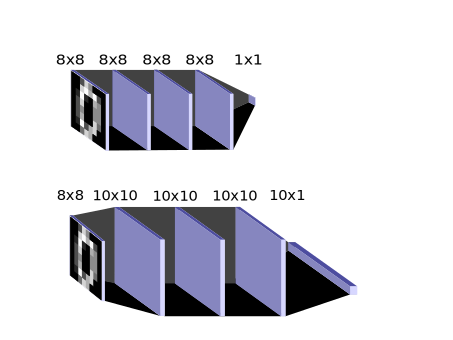
\includegraphics{../images/device_3d_view}
	\caption{(Top) An example configuration of the device for binary or one-versus-all classification on the digits dataset. (Bottom) An example configuration of the device for multi-label classification on the digits dataset. 
		The numbers along the top of both diagrams indicate the pixel dimensions of each layer. The leftmost layer is the input image, the three layers in the middle are the ‘hidden layers’, and the rightmost layer is the output layer. 
	}
\end{figure}

The device that I simulate is a box-like device that is made up of multiple layers. Each layer serves a different purpose and is a 2-D array of pixels. The first layer, the input layer, is simply a display for an image. The last layer is the output layer which is a 2-D array of detector pixels, and it acts similar to the output layer of an artificial neural network. The layers in between the input and output layers are called ‘hidden layers’, just like in artificial neural networks. These layers consist of 2-D arrays of translucent pixels, and the main basis of this device is that the transparency of these pixels can be controlled individually. This leads to similar behaviour to that of spatial light modulators, where an incoming wavefront (in this case the image) is modulated based on position. The total light intensity is measured at the output layer and is put through an activation function to give the final output of the device.

\section{Modeling the Device}
Some assumptions are made about the device. For one, I only consider light that has a path that can traced from a pixel in the input image directly to a pixel in the output layer. No reflection, refraction, or anything like that is considered in the model. The inverse square law that describes how the intensity of decreases with respect to distance is not considered. Pixel arrays in the device are assumed to have zero space between pixels, i.e. having a pixel fill factor of 100\%. Pixels are assumed to be square shaped. In other words, the model that I have implemented is a simple model.

The device is modeled with 3-D axis-aligned bounding boxes, and light paths are modeled via ray tracing. Each hidden layer has the transparency of its pixels set to a random value in the interval [0, 1].

The total light intensity of a given pixel in the output layer is calculated by taking the sum of the light intensity of all the incoming rays. For each pixel in the output layer, a separate ray is cast to each other pixel in the input image. Each ray initially takes on the value of the pixel in the input image that it is cast to. The ray is then checked for intersections in the hidden layers. The location that the ray intersects a layer also tells us which pixel the ray intersects. The light intensity of the ray is multiplied by the transparency value of this pixel. Once this has been done for each hidden layer we have the final light intensity value for the given ray. All the rays have their light intensity summed, giving the pre-activation value for the output pixel. Finally the output is transformed with an activation function. Although it is unclear if activation functions such as sigmoid or softmax can be implemented physically in the device, this step is necessary for training the weights (i.e. the transparency values of the pixels in the hidden layers). 

\begin{figure}
	\centering
	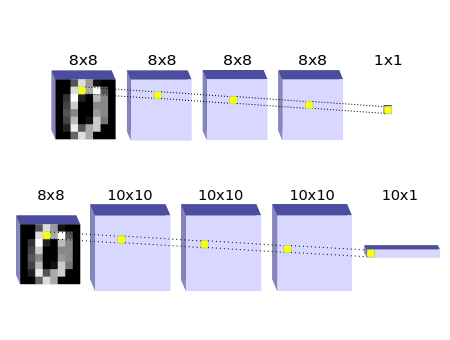
\includegraphics{../images/device_schematic}
	\caption{(Top) An example showing the path of a ray in the binary/one-versus-all classification configuration. (Bottom) An example showing the path of a ray in the multi-label classification configuration. The Yellow pixels denote where the ray would intersect each of the layers.
	}
\end{figure}

The output of a pixel in the output layer can be expressed as: 
$$I_p=\sigma(\sum_{i}\sum_{j}\alpha_{ij}X_{ij})$$
where $\sigma$ is an activation function, $X_{ij}$ is the value of the pixel located at row $i$ and column $j$ in the input image, and $\alpha_{ij}$ is the product of all the transparency values of the pixels in the hidden layers that are intersected by the ray cast from the output pixel $I_p$ to the pixel in the input image $X_{ij}$.

\section{Modeling the Device in Python}
My initial approach to calculating the output of the device was to calculate the light intensity of each of the rays individually, sum the light intensity values, and then apply the activation function. However this approach means that it is difficult to use libraries like TensorFlow or PyTorch and take advantage of their ability to automatically calculate gradients. The reason for this is that calculating the light intensity of each of the rays individually involves only scalar values and the calculations can not be vectorised.

Vectorising the ‘forward pass’ of the model is not entirely trivial, since it is possible that ray paths intersect the same pixel in a given layer and the number of pixels used varies between layers. 
My solution to this problem is to think of the forward pass more in terms of the rays. There are a fixed number of rays for each forward pass. Therefore the value of an output pixel can be thought of as the sum of the light intensity of $n$ rays, where $n$ is the number of pixels in the input image and thus the number of rays cast from the output pixel to the input image. Each of these rays intersect each hidden layer exactly once. Using the intersection points of the rays and hidden layers we can construct a matrix for each layer, where each element encodes the transparency value of the pixel that one of the rays intersect. These matrices act as the weight matrices used during a forward pass. The output of a pixel in the output layer can now be expressed as: 
$$I_p=\sigma(W\circ X)$$
where $W$ is the element-wise product of all of the weight matrices and $X$ is the input image and $\sigma$ is an activation function.

\section{Updating Pixel Values}
Due to the way that rays are cast from output pixels to the input image, some rays intersect the same physical pixel but these intersections are represented as separate elements in the weight matrices. During back-propagation these elements that share the same pixel may end up with different values. A physical pixel may only have one value at a time so these diverging values must be resolved to a single value. This is done by averaging the weights that correspond to the same hidden layer pixel.

Additionally, when there are multiple output pixels, each output pixel has a unique set of rays traced from itself to the pixels in the input image. This also means that the set of ray-pixel intersections are also unique to each output pixel, meaning each output pixel has a unique set of weight matrices. This is a problem because now not only between individual weights are pixel values shared, but also between multiple weight matrices. I took a similar approach to resolving the discrepancies between the individual weights that share the same physical pixel by averaging across the sets of weights. After applying the standard learning rule $w=w-\nabla J(w)$, the weights for each hidden layer pixel are summed and then divided by the number of rays that intersect the given hidden layer pixel. In summary, weights that share the same pixel are first averaged within each weight matrix separately, and then across each weight matrix for the given hidden layer.

\section{Experiments}
The dataset that I did my experiments on is the digits dataset, a scaled down version of the MNIST dataset that is distributed with the scikit-learn python package. This dataset consists of 1797 8x8 images. Prior to training the dataset is split into training and testing sets. During training, a validation set is split off from the training set. After training is complete the performance of the model is evaluated on the test set.

The model is trained with minibatch SGD, utilising early stopping and an adaptive learning rate. 
The performance on the validation set is monitored and when the validation loss does not decrease over a given number of epochs, the learning rate is decreased. Training is stopped early if the learning rate is decreased past the given limit.

For binary and one-versus-all classification, an output layer with two outputs are used, rather than just a single output. This is done for convenience so that no matter whether I am testing binary, one-versus-all, or multi-label classification I can use the same model with the same activation and loss functions.

For multi-label classification, the dataset is used as-is. However, for binary and one-versus-all classification the dataset is modified. For binary classification only images of zeros and ones are used. For one-versus-all classification, the labels are set to one for the instances of the digit zero, and set to zero for instances of the remaining digits.

The model achieves ~99\% accuracy when performing binary classification or one-versus-all classification. In multi-label classification the model achieves ~62\% accuracy. For more detailed results refer to the appenicies or the jupyter notebooks.

\section{Pixel Sharing}
The transparency value of a given pixel can possibly be represented in multiple weights across multiple different weight matrices, and output pixels end up sharing pixels. This has the effect that a hidden layer pixel that is shared by multiple rays/output pixels will never be able to reach its optimal value. The different output pixels are trying to classify different labels so they end up having conflicting interests. This conflict of interests is due to the averaging of weights detailed in section 4.

Ideally, each ray path from an output pixel to a pixel in the input image would have a unique path, and not share any pixels with other outputs/rays. The effect of pixel sharing can be reduced by doing two things: increasing the pixel density in the hidden layers, thus decreasing the chance that a pixel is shared; or placing the output pixels away from each other, thus reducing the amount of pixel sharing in the layers closer to the output layer. I have implemented the former, and it seems that having eight times the pixels in the hidden layer while maintaining the same overall relative scale of each layer provides the best performance. For multi-label classification it seems that increasing the pixel density to 16 is necessary. As for placing the output pixels away from each other, I have not yet tried this and this would be something to try in the future.

Another issue I believe to exist is the limited connectivity in the model. At present, only direct paths from the input image to the output image are considered. I noticed that in some implementations of vector-matrix multiplication using spatial light modulators, lenses would be used to distribute light across the pixel arrays. Such an addition may enable the device to approach the type of capabilities that a more typical artificial neural network has.

\section{Model Linearity}
As previously described, the output of a pixel in the output layer can be expressed as:
$$I_p=\sigma(\sum_{i}\sum_{j}\alpha_{ij}X_{ij})$$
Ignoring the activation function $\sigma$ for a moment, it seems like the model is linear. This can be seen by contrasting the above equation with the equation for a linear regression model:
\begin{equation*}
\begin{aligned}
y &= X\beta + \epsilon \\
  &= \sum_{i}\beta_i X_i + \epsilon
\end{aligned}
\end{equation*}
These equations are nearly identical, with the only major differences being an extra summation the absence of the term $\epsilon$ in the first equation. This poses the concern that the model will have limited abilities to learn complex functions.

\section{Future Work}
One thing that I have not tried is distributing, or dispersing, the output pixels so as to minimise the amount of pixel sharing. This may likely improve the models ability to learn as there will be less competition between outputs.

There is an issue with my current implementation, it is difficult to use the model with datasets other than those that can be loaded directly via scikit-learn’s dataset API. This is because for testing binary and one-versus-all classification I need to be able to manipulate the feature data and labels. This is a bit difficult with PyTorch’s data loader API. Also it is difficult to do the train, validation, test split that I am currently doing. 


It was initially thought that multiplying the light intensity by a transparency value would act like a ReLU non-linearity. However, due to the fact that there are no negative values in light intensity the clipping behaviour of the function for $x < 0$ does not occur, meaning that there is effectively no non-linearity in the model, i.e. the model is linear. There has been some research into optical implementations of various activation functions \cite{George:18, LI2019405}. One particular type of device comes to mind, saturable absorbers. These typically produce an output that is similar to the softplus activation function. For the simulation it may be worthwhile to try adding a softplus layer after each hidden layer to try introduce a nonlinearity into the model.

\section{Conclusion}
I have implemented a simulation of a device that can perform basic binary and one-versus-all classification, however the model seems to struggle with multi-label classification. The main issues with the device are pixel sharing and linearity, overcoming these issues should allow for better classification performance. Additionally, the performance of the model has only been tested on the digits dataset, so I think the next thing that should be on the project is to test the model on other datasets such as CIFAR-10.

\newpage
\bibliographystyle{plain}
\bibliography{report}

\newpage
\appendix
\section*{Appendix A: Classification Reports}
\begin{table}[h]
	\begin{tabular}{l|llll}
		& precision & recall & f1-score & support \\ \hline
		0 & 1.00 & 1.00 & 1.00 & 35 \\
		1 & 1.00 & 1.00 & 1.00 & 37  \\
		avg / total & 1.00 & 1.00 & 1.00 & 72 
	\end{tabular}
	\caption{Binary Classification Report.}
\end{table}

\begin{table}[h]
	\begin{tabular}{l|llll}
		& precision & recall & f1-score & support \\ \hline
		0 & 0.99 & 1.00 & 1.00 & 327 \\
		1 & 1.00 & 0.91 & 0.95 & 33  \\
		avg / total & 0.99 & 0.99 & 0.99 & 360 
	\end{tabular}
	\caption{One-Versus-All Classification Report.}
\end{table}

\begin{table}[h]
	\begin{tabular}{l|llll}
		& precision & recall & f1-score & support \\ \hline
		0 & 0.61 & 1.00 & 0.76 & 33 \\
		1 & 0.64 & 0.96 & 0.77 & 28 \\
		2 & 0.48 & 0.91 & 0.63 & 33 \\
		3 & 0.00 & 0.00 & 0.00 & 47 \\
		4 & 0.98 & 0.98 & 0.98 & 35 \\
		5 & 0.00 & 0.00 & 0.00 & 47 \\
		6 & 0.94 & 0.97 & 0.96 & 35 \\
		7 & 0.69 & 1.00 & 0.82 & 34 \\
		8 & 0.34 & 0.80 & 0.48 & 30 \\
		9 & 0.00 & 0.00 & 0.00 & 40 \\
		avg / total & 0.46 & 0.63 & 0.52 & 360
	\end{tabular}
	\caption{Multi-Label Classification Report. Note that the model did not correctly classify any instances of the digits three, five, or nine.}
\end{table}

\newpage
\section*{Appendix B: Confusion Matrices}

\begin{figure}[h!]
	\centering
	\scalebox{.75}{
		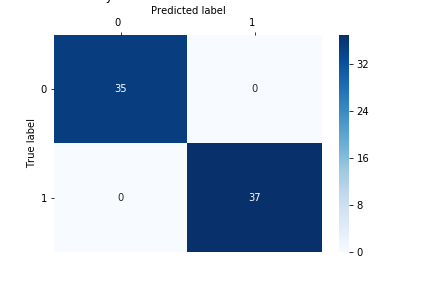
\includegraphics{../images/binary_classification_confusion_matrix}
	}
	\caption{Binary Classification Confusion Matrix.}
\end{figure}

\begin{figure}[h!]
	\centering
	\scalebox{.75}{
		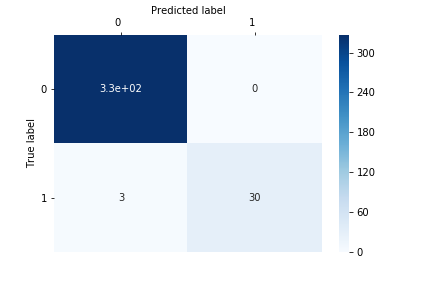
\includegraphics{../images/one-versus-all_classification_confusion_matrix}
	}
	\caption{One-Versus-All Classification Confusion Matrix.}
\end{figure}

\begin{figure}[h!]
	\centering
	\scalebox{.75}{
		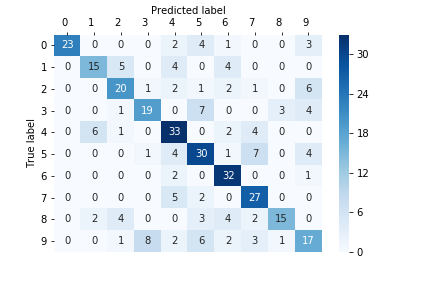
\includegraphics{../images/multi-label_classification_confusion_matrix}
	}
	\caption{Multi-Label Classification Confusion Matrix. Note that the model did not correctly classify any instances of the digits three, five, or nine.}
\end{figure}
\clearpage

\newpage
\section*{Appendix C: Sample of Predictions}

\begin{figure}[h!]
	\centering
	\scalebox{.75}{
		\makebox[\textwidth]{
			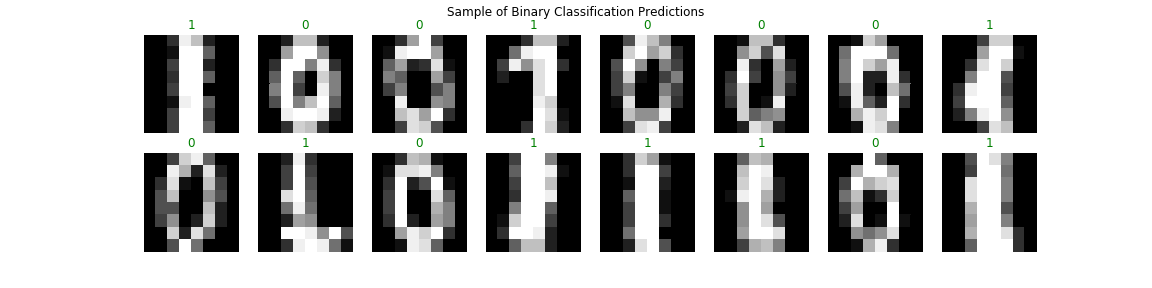
\includegraphics[width=\paperwidth]{../images/binary_classification_prediction_sample}
		}
	}
	\caption{Sample of Binary Classification Predictions. Green indicates a correct classification.}
\end{figure}

\begin{figure}[h!]
	\centering	
	\scalebox{.75}{
		\makebox[\textwidth]{
			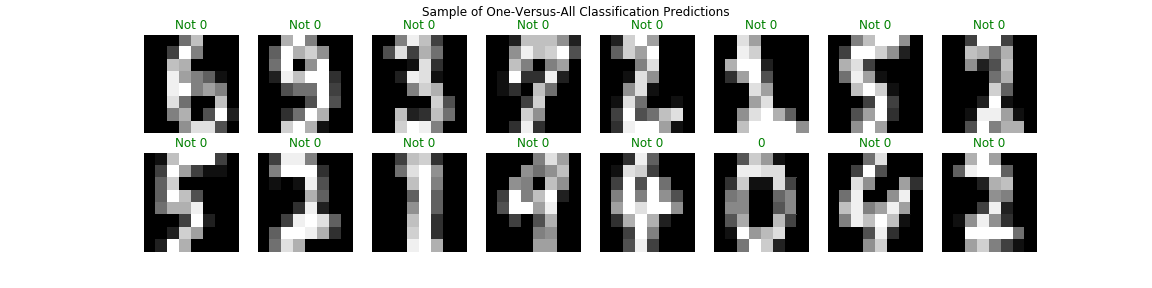
\includegraphics[width=\paperwidth]{../images/one-versus-all_classification_prediction_sample}
		}
	}
	\caption{Sample of One-Versus-All Classification Predictions. Green indicates a correct classification.}
\end{figure}

\begin{figure}[h!]
	\centering	
	\scalebox{.75}{
		\makebox[\textwidth]{
			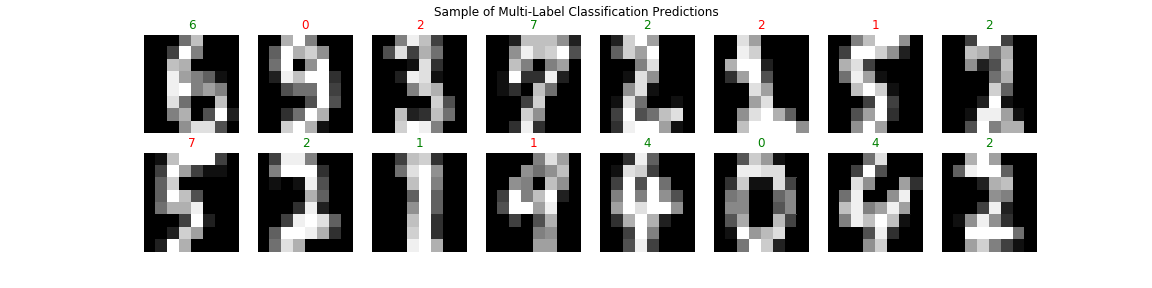
\includegraphics[width=\paperwidth]{../images/mutli-label_classification_prediction_sample}
		}
	}
	\caption{Sample of Multi-Label Classification Predictions. Green indicates a correct classification, and red indicates an incorrect classification.}
\end{figure}

\newpage
\section*{Appendix D: Hidden Layer Pixel View}

\begin{figure}[h]
	\centering
	\scalebox{.85}{	
		\makebox[\textwidth]{
			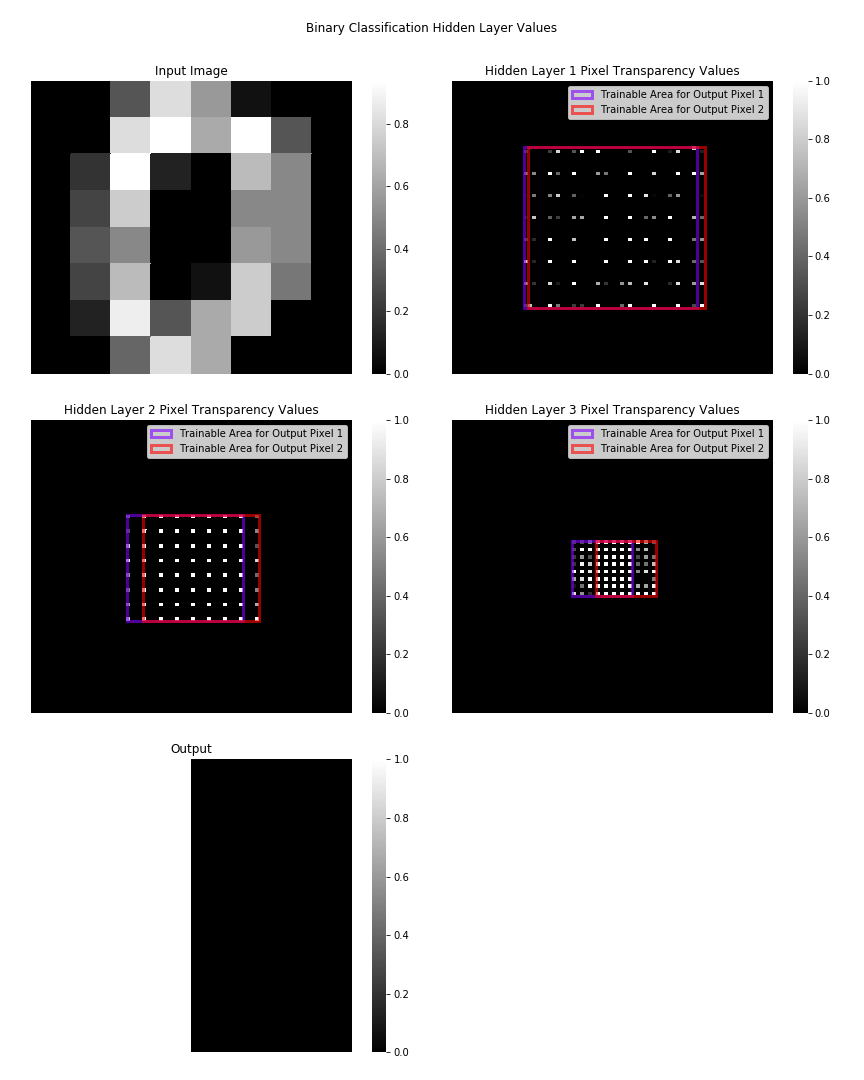
\includegraphics[width=\textwidth, height=\textheight, keepaspectratio]{../images/binary_classification_hidden_layer_values}
		}
	}
	\caption{A series of plots showing a sample input image (top left), the hidden layers and the area of trainable pixels (top right, middle left, middle right), and a sample output (bottom left) from a classifier trained for binary classification.}
\end{figure}

\begin{figure}
	\centering
	\makebox[\textwidth]{
		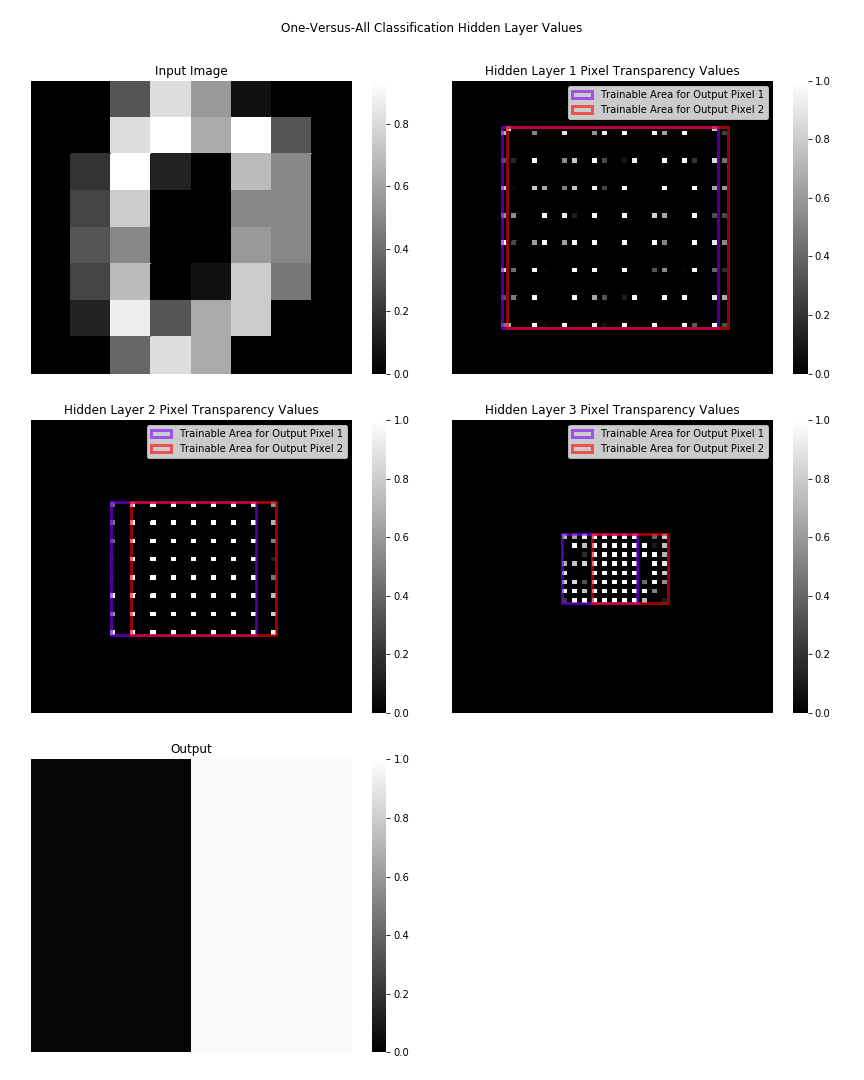
\includegraphics[width=\textwidth, height=\textheight, keepaspectratio]{../images/one-versus-all_classification_hidden_layer_values}
	}
	\caption{A series of plots showing a sample input image (top left), the hidden layers and the area of trainable pixels (top right, middle left, middle right), and a sample output (bottom left) from a classifier trained for one-versus-all classification.}
\end{figure}

\begin{figure}
	\centering
	\makebox[\textwidth]{
		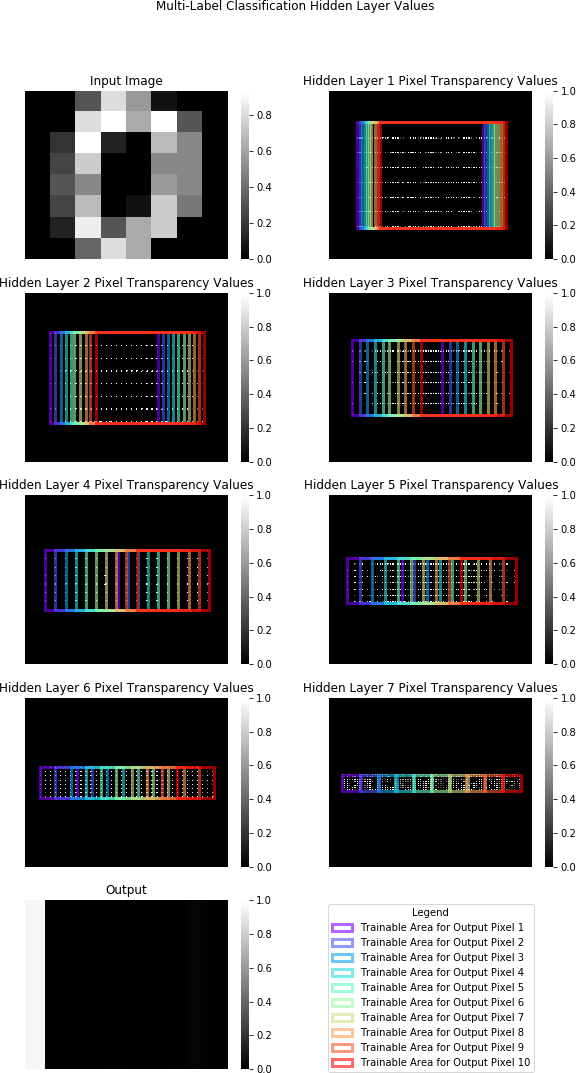
\includegraphics[width=\textwidth, height=0.9\textheight, keepaspectratio]{../images/multi-label_classification_hidden_layer_values}
	}
	\caption{A series of plots showing a sample input image (top left), the hidden layers and the area of trainable pixels (top right, middle left, middle right), and a sample output (bottom left) from a classifier trained multi-label classification.}
\end{figure}

\end{document}          
